 \documentclass[12pt]{article}

\usepackage{sbc2003}

\usepackage{graphicx,url}

\usepackage[brazil]{babel}   
\usepackage[utf8]{inputenc}
%\usepackage[latin1]{inputenc}

%Para notas
\usepackage{todo}

\usepackage{comment}

% Para estilização dos códigos
\usepackage{minted}
\renewcommand{\listingscaption}{Código}

% Para lista em linhas
\usepackage{paralist}

% Identar primeiros parágrafos
\usepackage{indentfirst}
\sloppy
\title{Termpot: criação, edição e execução de funções no navegador em tempo de execução .}

\author{Guilherme Lunhani\inst{1}
        \and 
        Flávio Luiz Schiavoni\inst{2}}

\address{Instituto de Artes e Design --
         Universidade Federal de Juiz de Fora \\
         Juiz de Fora, MG
         \email{gcravista@gmail.com, ttonmeister@gmail.com}
         \nextinstitute
         Departamento de Computação --
         Universidade Federal de São João Del Rei \\
         São João Del Rei, MG
         \email{fls@ufsj.edu.br}
}
\begin{document} 

\maketitle

%%%%%%%%%%%%%%%%%%%%%%%%%%%%%%%%%%%%%%%%%%%%%%%%%%%%%%%
% Google Translate; fiz p agilizar, mas preciso arrumar
% Deve ter coisas sem sentido
%%%%%%%%%%%%%%%%%%%%%%%%%%%%%%%%%%%%%%%%%%%%%%%%%%%%%%%

\begin{abstract}
This panel reports the development of a sound synthesis program, Termpot. The Web Audio API technology was used in a reinterpretation of a \cite{mathews_groove_1970}'s work, GROOVE. The resulting work is still in its infancy, but allows create and edit sound functions at runtime, in a web browser.
\ \\
\textbf{Keywords}: GROOVE; Web Audio API; DSP.
\end{abstract}


\begin{resumo} 
Este painel reporta o desenvolvimento de um programa de síntese sonora, Termpot. A tecnologia Web Audio API foi usada em uma reinterpretação de um trabalho de \cite{mathews_groove_1970}, GROOVE. O trabalho resultante ainda é incipiente, mas possibilita criar e editar funções no tempo de execução, em um navegador web.
\ \\
\textbf{Palavras-chave}: GROOVE; Web Audio API; DSP.
\end{resumo}

%%%%%%%%%%%%%%%%%%%%%%%%%%%%%%%%%%%%%%%%%%%%%%%%%%%%%%%
% TRAMPO: Tratar como um poster de 4 páginas, conforme 
% PARECER.md
%%%%%%%%%%%%%%%%%%%%%%%%%%%%%%%%%%%%%%%%%%%%%%%%%%%%%%%

\section{Introdução}\label{sec:introducao}

% - Qual é a da coisa? (sintese c webaudio)
% - como a coisa funciona? 
%   - como um ou outro fez funcionar
%   - nosso jeito de funcionar

% -----------------------------------------------
 % http://www.charlie-roberts.com/pubs/Gibber_charles_roberts_icmc_2012.pdf


A síntese sonora em \emph{web browsers} é sumarizada por \cite{w3c_web_2012,roberts_web_2013-,wyse_viability_2014}.\cite{srikumar_tamming_2013} exemplifica uma concatenação de \emph{nós de áudio} em um grafo de DSP. \ Três nós diferentes são representados na figura \ref{fig:chime}. Existe um outro nó (figura \ref{fig:scriptprocessor}) que possibilita definir formas de ondas customizadas. O \emph{Termpot} explora este nó, e delega, como o \emph{wavepot} \footnote{Disponível em \url{https://www.github.com/wavepot/wavep0t}}, as customizações para um(a) improvisador(a), que cria suas próprias \emph{funções de transferência} e \emph{interfaces de controle} \cite{mathews_groove_1970}.

\begin{figure}[!h]
\centering
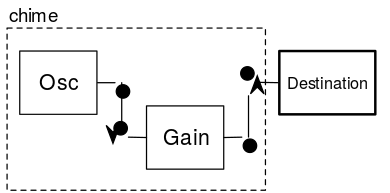
\includegraphics[scale=0.3]{chime.png}
\caption{Estrutura básica de um sintetizador webaudio. \emph{OscilatorNode}, \emph{GainNode} e \emph{DestinationNode} (alto-falante). \textbf{Fonte}: \cite{srikumar_tamming_2013}}
\label{fig:chime}  
\end{figure}


\begin{figure}[!h]
\centering
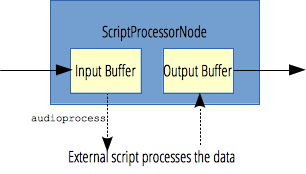
\includegraphics[scale=0.6]{WebAudioScriptProcessingNode.png}
\caption{``A interface do \emph{ScriptProcessorNode} permite a geração, processamento ou análise de áudio usando JavaScript''. \textbf{Fonte}: \cite{w3c_web_2012}}
\label{fig:scriptprocessor} 
\end{figure}


\section{Trabalho relacionado: GROOVE}

Reinterpretamos um trabalho de \cite{mathews_groove_1970}, o sistema GROOVE, \emph{Generated Real-time Operations On Voltage-controlled Equipment}. A compositora Laurie Spiegel (figura \ref{fig:groove}) sumariza suas as características, durante a produção de \emph{The Expanding Universe} (1975)\footnote{Disponível em \url{https://www.youtube.com/watch?v=dYUZmsfm4Ww}.}, entre as salas 2D-506 da Bell Labs (contendo o computador DDP-224) e a sala analógica 2D-562 (laboratório de Mathews):

\begin{quote}
\small{Todas as músicas no GROOVE eram representadas na memória digital como funções abstratas do tempo, séries paralelas de dois pontos, cada ponto sendo um instante no tempo e um valor instantâneo. A taxa de amostragem para essas funções, usada principalmente como controle de voltagem, era cronometrada por um grande e antiquado oscilador analógico que era normalmente fixado em 100 Hertz, cada ciclo do oscilador pulsando à frente do código, o computador lia, em cada uma das funções, naquele ponto do tempo, todos dispositivos de entrada e executava todas amostras. (\ldots) Tínhamos uma pequena caixa com 4 potenciômetros e quatro chaves (alternadores fixados onde você os colocava) e dois botões de disparo.} \footnote{Tradução de \emph{All music in GROOVE was represented in digital memory as abstract functions of time, parallel series of point pairs, each point being an instant in time and an instantaneous value. The sampling rate for these functions, which would be used mostly as control voltages, was clocked by a big old-fashioned analog oscillator that was usually set to 100 Hertz, each cycle of the oscillator pulsing one run through the code, the computer reading all of the real time input devices and playing of all of the samples at that time point in each of the time functions. (\ldots)  We had a small box with 4 knobs, 4 set switches (toggles that stay where you put them) and 2 momentary-contact push buttons on it.}}
\end{quote}

\begin{figure}[!h]
  \begin{center}
  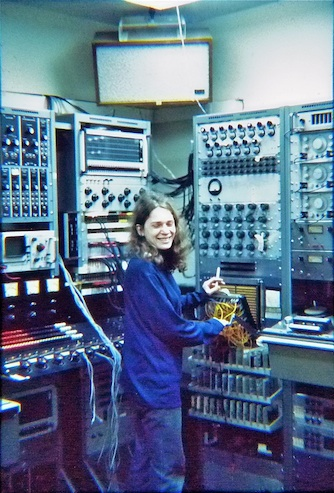
\includegraphics[scale=0.5]{./spiegel.jpg}
  \caption{\small Laurie Spiegel configurando a saída analógica do GROOVE, durante a produção de \emph{The Expanding Universe}. \textbf{Fonte}: \cite{spiegel_expanding_1975}.}
  \label{fig:groove}
  \end{center}
\end{figure}

\section{Metodologia de desenvolvimento}

\begin{inparaenum}[\itshape 1)\upshape]
\item Customização um emulador terminal \emph{Ptty.js} (\footnotesize \url{http://code.patxipierce.com/jquery-plugin/ptty/} \normalsize).
\item Definição de um ambiente interno, baseado no ambiente \emph{Wavepot}, controlador do \emph{ScriptProcessorNode}.
\item Definição de comandos deste ambiente interno: inspeção de funções, definição de novas funções, tocar, parar, pausar, gravar e download, criação de controles gráficos (\emph{jQueryUI}) e gravação (\footnotesize \url{https://github.com/mattdiamond/Recorderjs/blob/master/recorderWorker.js} \normalsize).
\end{inparaenum}


%\section{Trabalhos relacionados}\label{sec:trabalhos}

Nesta seção apresentaremos a API webaudio e as ferramentas / frameworks Gibber e Wavepot.

\subsection*{WebAudio API}\label{sec:webaudioapi}

O primeiro trabalho relacionado é a própria API Webaudio e seu nó especial para processamento de sinais (\emph{ScriptProcessorNode}), que permite os três trabalhos serem co-relacionados.
Uma característica lógica do ScriptProcessorNode é sua linearidade, possibilitando calcular cada amostra do vetor de saída de maneira direta.
Isto permite \begin{inparaenum}[\itshape a)\upshape]
\item uma possível redução no custo  computacional para sínteses de ondas complexas;
\item a definição matemática de um vetor de saída a partir da definição de uma função; e
\item a criação de qualquer tipo de nó de processamento de áudio\end{inparaenum}.
No Código \ref{code:ex1} demonstramos uma simples utilização desta API.

\begin{listing}
\begin{minted}[linenos,frame=lines,framesep=2mm,fontsize=\scriptsize]{javascript}
// Chrome ou firefox?
var context = new AudioContext();
var node = context.createScriptProcessor(1024, 0, 1);

// DSP
var noise = function(amplitude){
    var sample = Math.random() * 2 - 1
    return sample * amplitude
}

node.onaudioprocess = function(e) {
  var output = e.outputBuffer.getChannelData(0);
  for (var i = 0; i < data.length; ++i) {
    output[i] = noise(0.5)
  }
}
node.connect(context.destination); // TOCAR
node.disconnect(); // PARAR
\end{minted}
\caption{Exemplo de utilização do ScriptProcessorNode}
\label{code:ex1}
\end{listing}

Esta abordagem é conveniente do posto de vista musical entre as linhas e 6-9 do Código \ref{code:ex1}. Para o músico, o restante pode ser  especificidade técnica que pode desviar a atenção composicional. Nesse sentido, o \emph{Gibber} e \emph{Wavepot} oferecem soluções possíveis para aqueles que se interessam em manter um controle dos algoritmos musicais.

% http://lammax.lnu.se/ubimus/wp-content/uploads/sites/5/2015/03/ubimus6_submission_2.pdf
% -----------------------------------------------
% -----------------------------------------------
% -----------------------------------------------
% -----------------------------------------------
% -----------------------------------------------
% -----------------------------------------------
% -----------------------------------------------
\subsection*{Gibber}

O Gibber\footnote{Disponível em \url{http://gibber.mat.ucsb.edu/}.} é descrito por \cite{roberts_gibber:_2012} como um ambiente de \emph{live coding}\footnote{Para mais informações sobre a prática \emph{live coding}, sugerimos a leitura dos seguintes autores: \cite{collins_live_2003,ward_live_2004,collins_live_2007,rohrhuber_improvising_2009,magnusson_algorithms_2011,collins_origins_2014}. Seu foco está em tornar a atividade de codificação produtiva do ponto de vista musical.}. Possui um \emph{layout} de abas divididas entre: \begin{inparaenum}[\itshape 1)\upshape]
\item editor de texto;
\item um \emph{canvas} contendo imagens resultantes dos códigos visuais;
\item um navegador do aplicativo, contendo rotinas diversas;
\item alternador de códigos sonoros e códigos visuais
\item navegador de códigos musicais do servidor;
\item um console de informações;
\item \emph{login} para um círculo de contas restritas ao aplicativo.
\end{inparaenum}Nosso interesse maior tange ao item 1, e em como o código escrito processa os sinais digitais.Uma outra abordagem técnica, descrita na próxima sessão,  elucida as linhas 136-175 do código-fonte da máquina de áudio do \emph{Gibber}, \emph{Gibberish}\footnote{Disponível em \url{https://github.com/charlieroberts/Gibberish}.}. Descartaremos portanto o estudo do \emph{Gibber} para focar no \emph{Wavepot}.

\begin{figure}[h]
\centering
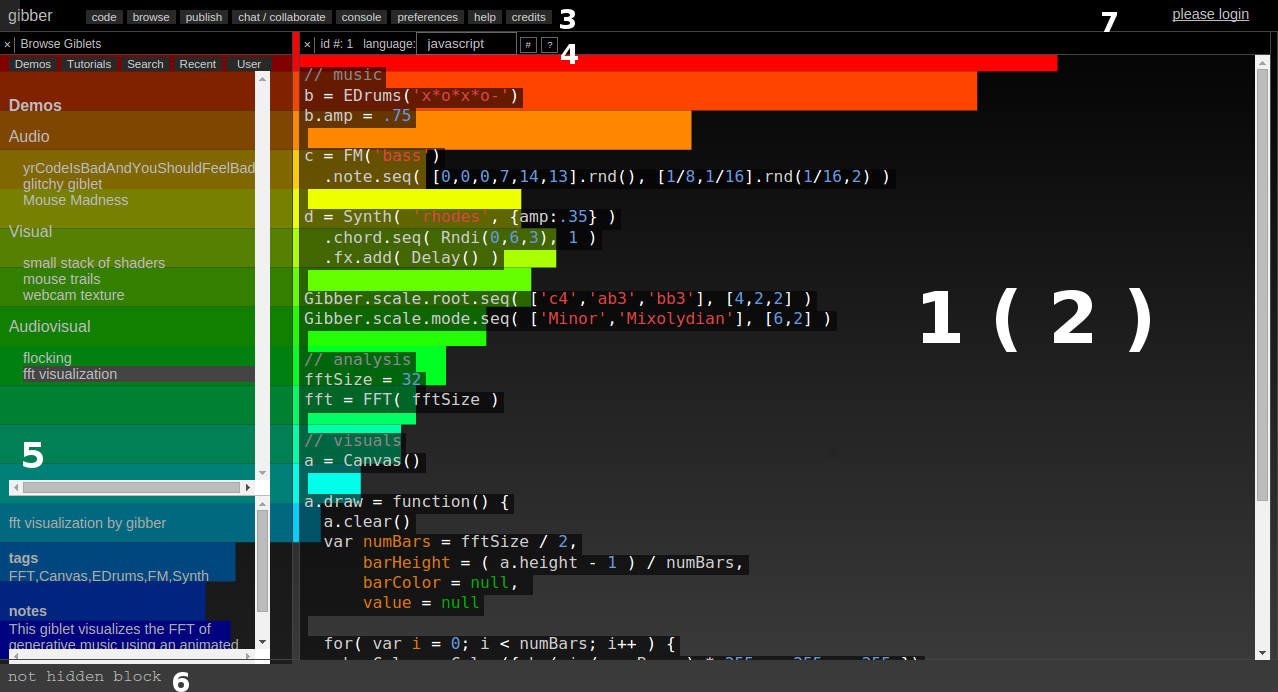
\includegraphics[scale=0.35]{gibber.png}
\caption{Aplicativo \emph{Gibber}. \textbf{Fonte}: \protect\url{http://gibber.mat.ucsb.edu}}
\label{fig:gibber}
\end{figure}


% -----------------------------------------------
% -----------------------------------------------
% -----------------------------------------------
% -----------------------------------------------
% -----------------------------------------------
% -----------------------------------------------
% -----------------------------------------------
\subsection*{Wavepot}

É uma \emph{webaudio-daw}\footnote{\emph{Webaudio Digital Audio Workstation} disponível em \url{https://github.com/wavepot/wavep0t/blob/master/index.js}.}.
Esta ferramenta possui as seguintes características:\begin{inparaenum}[\itshape 1)\upshape]
\item layout que expõe a partitura-programação \cite{fenerich_marulho_2014} do lado esquerdo. Geralmente é dividida em dois editores, semelhante ao método \emph{instrumento-orquestra}~\cite{mathews_digital_1963,di_nunzio_genesi_2010};
\item do lado direito, controles de tocar, parar e gravar, menu de exemplos, módulos, músicas, ajuda, alternáveis;
\item compartilhamento e atualizações dos códigos através do \emph{Github};
\item um analisador gráfico da formas de onda resultantes;
\item uma lista de cabeçalhos dos códigos abertos;
\item um console de retorno de informações.
\end{inparaenum}

\begin{figure}[h]
\centering
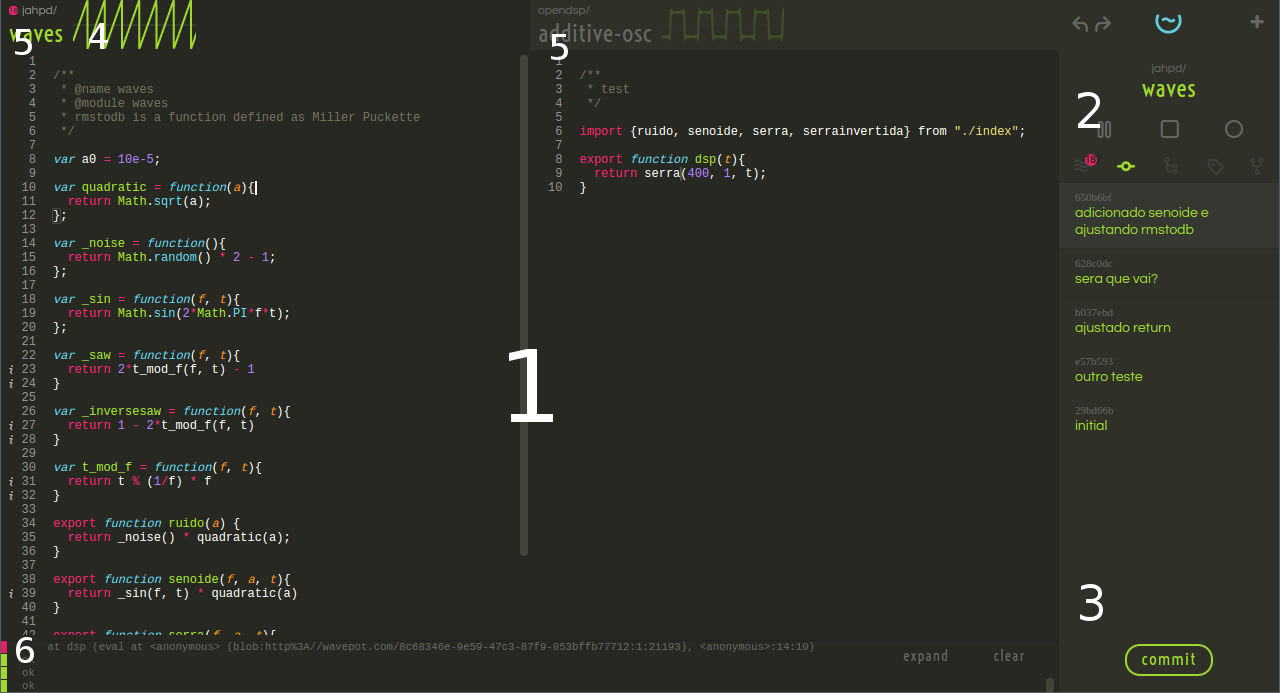
\includegraphics[scale=0.35]{wavepot.png}
\caption{Aplicativo \emph{Wavepot}. \textbf{Fonte}: \protect\url{https://www.wavepot.com}}
\label{fig:wavepot}
\end{figure}

Existe um modo padronizado de programação que requer observações. A primeira é que o improvisador utilize uma variável $t$. Esta variável pode ser descrita como a fase de um tempo discretizado $td=1/sampleRate$. É util para calcular formas de ondas diversas. No exemplo \ref{code:ex2} demonstramos o uso do $t$ para criar uma senóide. A segunda exige a utilização do \emph{token} \verb|export| antes de definir a função $dsp$.


\begin{listing}
\begin{minted}[linenos,frame=lines,framesep=2mm,fontsize=\scriptsize]{javascript}
var noise = function(amplitude){
    return (Math.random() * 2 - 1) * a;
}

var sin = function(freq, amp, t){
    return Math.sin(Math.PI * 2 * freq * t) * a
}

export function dsp(t){
    return noise(1) * sin(1, 1, t)
}
\end{minted}
\caption{Sintetizando um ruído controlado por um LFO senoidal}
\label{code:ex2}
\end{listing}

% -----------------------------------------------


\subsection{Comparação de trabalhos relacionados}

Para entender a relação entre estas duas ferramentas, montamos um quadro comparativo a partir de alguns parâmetros: tipo de música realizada nos códigos exemplares,  suporte a vídeo, compilação em tempo de execução, estratégia de partitura-programação,  biblioteca de síntese e suporte ao compartilhamento dos códigos. Esta comparação é apresentada na Tabela \ref{tab:comparacao}.
Em ambos os casos, ocorre a tradução de um código em linguagem \emph{javascript} para o processamento de áudio.
Uma discussão musicológica envolve entre outros fatores, um tipo de música tocado em eventos conhecidos como \emph{algoraves}~\cite{collins_algorave:_2014,mori_analysing_2015}.

\renewcommand{\arraystretch}{1.35} %Espacamento entre as linhas

\begin{table}[ht!]
\caption{Tabela comparativa de funcionalidades entre o \emph{Gibber} e o \emph{Wavepot}.}
    \begin{tabular}{ p{4cm} | p{5cm} | p{5cm}}
    \hline 
    \hline 
    \textbf{Característica}      & \textbf{Wavepot}  & \textbf{Gibber} \\
    \hline 
    \hline 
    
    Linguagem de programação & Javascript & Javascript \\
    \hline
    
    Tipo de música      & Algorave & Algorave + glitch/noise\\
    \hline
    
    Vídeo               & Não      & \small Sim - Síntese de imagens 2D e 3D através de uma implementação OpenGL. Podem sincronizar com alguns parâmetros sonoros.    \\
    \hline
    
    Compilação em tempo de execução & \small Sim -- qualquer edição no código é automaticamente reconhecido enquanto estiver sendo processado algum sinal de áudio. & \small Sim -- o executante musical deve utilizar teclas de atalho para requerir ao servidor o processo de compilação. \\
    \hline
    
    Partitura-programação      & \small Editor de texto desenvolvido com a biblioteca \emph{Ace}\footnotemark \footnote{Disponível em \url{http://ace.c9.io/#nav=about}.} em duas partes, subdividido pelos autores deste artigo como \emph{instrumentais} e \emph{orquestrais}  & \small Editor de texto, com alternância dos códigos sonoros (\emph{javascript}) e códigos visuais (\emph{OpenGL}) \\
    \hline

    Biblioteca de síntese  & 
    $Audio-process$\footnote{Disponível em \url{https://github.com/wavepot/wavep0t/blob/master/index.js}.} & 
    Gibberish\footnote{Disponível em \url{https://github.com/charlieroberts/Gibberish/blob/master/scripts/gibberish.js}.}    \\
    \hline
    
    Criação de novos módulos em tempo de execução  & \small Sim -- o improvisador pode criar funções através de variáveis ou as palavras-chave $export default function$ & Não \\
    \hline
    Compartilhamento de códigos &
    O usuário pode criar, ou reutilizar módulos e músicas, através da rede social $Github$  & 
    Códigos musicais podem ser publicados no servidor do Gibber abrindo uma conta no próprio site. \\
    \hline 
    Elementos de GUI &
    \small Não existe na versão oficial, no entanto um experimento foi desenvolvido para sincronizar a máquina de síntese \emph{Wavepot} com controladores MIDI\footnote{A discussão inteira está disponível em \url{https://groups.google.com/forum/?hl=pt-BR#!topic/wavepot/i5H7rRvcdpQ}, enquanto o exemplo está disponível em \url{http://boxbase.org/sequencer/}.}. A GUI servia, portanto, para averiguar o funcionamento do MIDI.  &
    Sim -- Pode ser utilizado com a biblioteca \emph{Interface.js}\footnote{} \\
    \hline
    \hline
    \end{tabular}
\label{tab:comparacao}
\end{table}


%Enquanto o primeiro possui um código aberto desde 16 de Junho de 2012\footnote{Disponível em \url{https://github.com/charlieroberts/Gibberish/commit/fec69715908505869e6fa8e7fca4e5eb08ea1f4e}.}, o segundo abriu parcialmente o código no começo de Setembro\footnote{Disponível em \url{https://github.com/wavepot/wavep0t/commit/ed988a9512bb5244b500cfbbeae77f94741856c5}.}
\section{Termpot}\label{sec:termpot}

O Termpot (ver Figura \ref{fig:termpot}) é um ambiente para improvisação de luteria composicional \cite{iazzetta_musica_2009,soares_luteria_2015}, mais especificamente, um ambiente \emph{web} de \emph{livecoding}. Adapta o ambiente \emph{Wavepot} (apresentado na nota-de-rodapé 2 da Seção \ref{sec:introducao}) para um emulador de terminal, controlado pela linguagem \emph{coffeescript}\cite{burnham2011coffeescript}\footnote{\url{http://coffeescript.org/}, acessado em \today.}. O ambiente possibilita a improvisação de códigos com a extensão média de uma linha (ver Código \ref{code:resultado1}). 

\begin{figure}[!h]
\centering
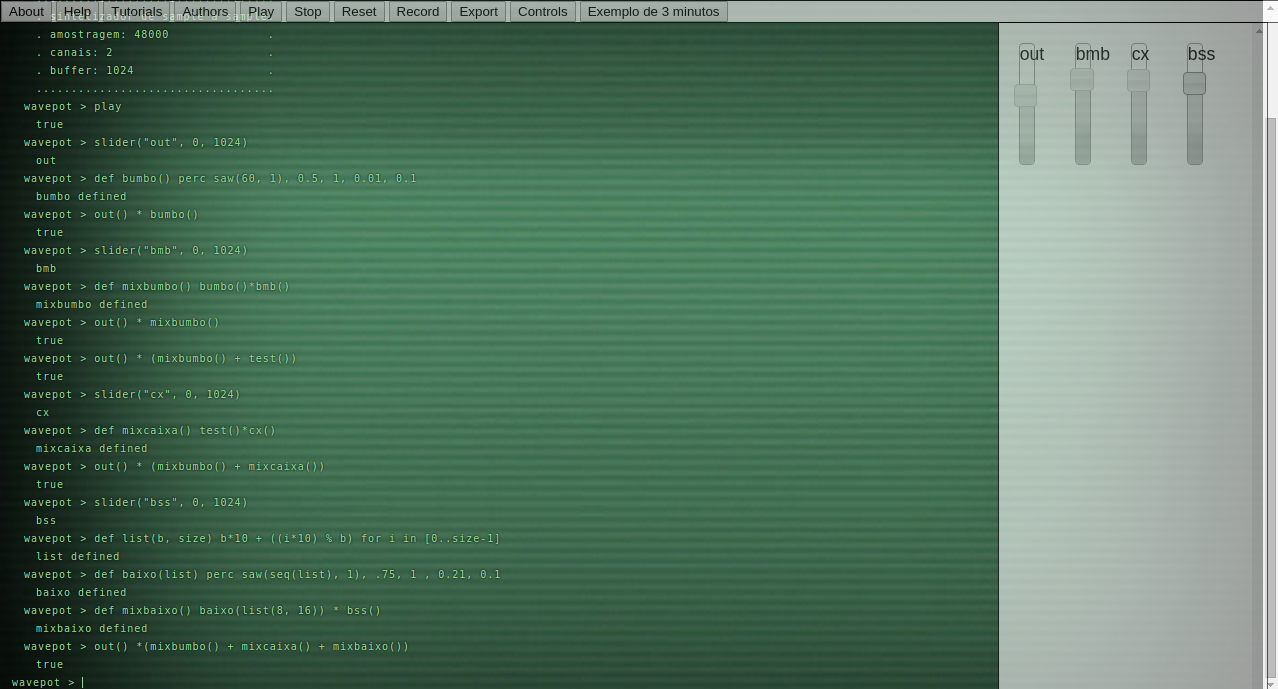
\includegraphics[scale=0.35]{termpot.png}
\caption{Aplicativo \emph{Termpot}. \textbf{Fonte}: autores.}
\label{fig:termpot}
\end{figure}

\begin{listing}
\begin{minted}[linenos,frame=lines,framesep=2mm,fontsize=\scriptsize]{javascript}
.........................................
. Virtual machine started at             .
. Thu Sep 03 2015 13:32:15 GMT-0300 (BRT).
. type help for instructions             .
..........................................
$\$$ |
$\$$ wavepot 1024
..................................
. sintetizador de sample a sample. 
. amostragem: 44100              .
. canais: 2                      .
. buffer: 1024                   .
..................................
wavepot > play
wavepot > 0.71 * sin 440, sin(330, sin(220, 0.5)
true
\end{minted}
\caption{Console do \emph{termpot} aguardando dados de entrada do improvisador; o improvisador inicia o ambiente wavepot com um buffer de 1024 pontos flutuantes; o improvisador inicia o processamento de áudio; o improvisador define o processamento de áudio de uma cascata de Modulção de amplitude.}
\label{code:resultado1}
\end{listing}

Em tese, é possível criar sonoridades semelhantes ao \emph{Wavepot}. Porém, dado o curto tempo de desenvolvimento, pré-definimos apenas ruído (branco), senóide, dente-de-serra, triangular, pulso, envelope e sequenciamento.

É possível prototipar rapidamente novas funções para encapsular novas funcionalidade sonoras ao ambiente.

\begin{listing}
\begin{minted}[linenos,frame=lines,framesep=2mm,fontsize=\scriptsize]{javascript}
wavepot > def tresAM(f, f1, f2, a) a * sin f, sin(f1, sin(f2, 0.5)
true
wavepot > inspect tresAM
var tresAM;

tresAM = function(f, f1, f2, a) {
  return a * sin(f, sin(f1, sin(f2, 0.5)))
};
wavepot > tresAM 440, 330, 220, 0.71 
\end{minted}
\label{code:resultado2}
\end{listing}

Além da atividade de síntese, elaboramos uma maneira para a criar e utilizar GUIs de controle (\emph{sliders}), como uma mesa de som (ver Código \ref{code:resultado3}

\begin{listing}
\begin{minted}[linenos,frame=lines,framesep=2mm,fontsize=\scriptsize]{javascript}
wavepot > slider("left", 0, 1024)
true
wavepot > slider("right", 0, 1024)
true
wavepot > stereo sin(440,0.5)*left(), sin(330, 0.5)*right()
true
\end{minted}
\caption{Exemplo de código do Wavepot}
\label{code:resultado3}
\end{listing}


Uma característica singular do \emph{Wavepot} original, é a possibilidade de separação da programação-partitura em dois arquivos, muito semelhante ao método \emph{Instrumento-Orquestra} descrito por Max Mathews e utilizado no CSound \cite{mathews_digital_1963, di_nunzio_genesi_2010}.
Isso é possível adicionando um marcador $@module$ aos comentários iniciais de um código.
Desta forma, serão reconhecidos dois arquvivos durante a performance de improvisação: $index.js$ e $test.js$.
O primeiro permite elaborar os instrumentos, enquanto o segundo realiza o DSP (teste).

Já no Termpot, buscamos utilizar outro método de codificação focado em uma abordagem mais performática.


Arriscamos a comentar uma inspiração no GROOVE de \cite{mathews_groove_1970,nunzio_groove_2010}, quando este propõe a criação de novas funções em tempo de execução. Ao mesmo tempo em que utilizamos a biblioteca \emph{Ptty.js} dando ao \emph{Termpot} as características de um emulador de terminal no que tange a utilização de comandos em tempo de execução, como em um terminal, integrado com controles manuais.
Por esta razão, acreditamos que esta ferramenta é inspirada no conceito de compor, memorizar, editar e controlar funções do tempo, algoritmicamente e manualmente~\cite{mathews_groove_1970}.


%\subsection*{Metodologia de desenvolvimento}

%Para a implementação, três tarefas foram necessárias: \begin{description}
%\item[1) Customizar um emulador terminal]
%\item Utilizamos a biblioteca \emph{Ptty.js} é uma biblioteca documentada e pode ser facilmente implementada seguindo instruções de seu arquivo \emph{README}. É baseada em jQuery e permitiu uma rápida prototipação.
%\item[2) Implementar um ambiente de síntese sonora integrado ao emulador]
%\item Uma das facilidades do \emph{Ptty} é definir ambientes; elaboramos um ambiente que controla a \emph{Web Audio API} nos moldes descritos na Seção 2.
%\item[3) Comandos diversos]
%\item Ajuda, inspeção de funções, definição de novas funções, tocar, parar, pausar, gravar e download e criação de controles gráficos. Para gravação, utilizamos o \emph{recorderWorker.js}\footnote{\url{https://github.com/mattdiamond/Recorderjs/blob/master/recorderWorker.js}.} de Matt Diamond.
%\end{description}

%\section{Resultados}\label{sec:resultados}

Ao iniciar a página, o improvisador é colocado diante de emulador de terminal. Para obter ajuda de uso, o improvisador pode digitar $help$.
O comando \emph{Wavepot} pode ser executado com um argumento, que é o tamanho do \emph{buffer}.
Valores válidos devem ser potência de dois (2), entre 256 e 16384, sendo que o padrão é 1024 (ver Código \ref{code:resultado1}).
Alguns comando gerais como \emph{play}, \emph{stop}, \emph{pause} e \emph{reset} são utilizados para execução. 
\emph{Record} e \emph{export} para gravação de uma performance e exportação desta performance para um arquivo de extensão \emph{.wav}.

O comando \emph{play} inicia uma incrementação da variável $t$; o comando $pause$ "congela" $t$ e coloca o sintetizador em estado suspenso; $reset$ redefine $t=0$, porém não congela a incrementação. $Stop$ realiza a mesma tarefa que $pause$, porém desliga o sintetizador.

\begin{listing}
\begin{minted}[linenos,frame=lines,framesep=2mm,fontsize=\scriptsize]{javascript}
.........................................
. Virtual machine started at             .
. Thu Sep 03 2015 13:32:15 GMT-0300 (BRT).
. type help for instructions             .
..........................................
$\$$ wavepot 1024
..................................
. sintetizador de sample a sample. 
. amostragem: 44100              .
. canais: 2                      .
. buffer: 1024                   .
..................................
wavepot > play
wavepot > sin 440, 0.5
true
\end{minted}
\caption{Console do \emph{wavepot} aguardando dados de entrada do improvisador.}
\label{code:resultado1}
\end{listing}

\subsection*{Realizando sínteses}

A síntese no ambiente \emph{wavepot} é realizada fornecendo uma função que retorne dados entre -1.0 e 1.0, atuando diretamente sobre a linha 8 do exemplo apresentado na Seção \ref{sec:webaudioapi}.
No exemplo apresentado no Código \ref{code:resultado7}, ao utilizar a expressão \verb|Math.random() * 2 - 1|, a cada intervalo de tempo $td=1/SR$ (taxa de amostragem), um novo número randômico é mapeado entre o intervalo permitido, resultando em um ruído branco.

Uma maneira de simplificar o cálculo de um ruído, é definí-lo em uma função, como no Código \ref{code:ex1}. 

Já existe no aplicativo uma função \verb|noise(a)|.
Porém, como o objetivo é demonstrar seu uso, exemplificamos o processo ainda no Código \ref{code:resultado7}.
Ao  utilizar o \emph{token} \verb|def|, definimos em tempo de execução uma função chamada \verb|ruidobranco(a)|.

\begin{figure}[ht!]
\begin{minted}[linenos,frame=lines,framesep=2mm,fontsize=\scriptsize]{javascript}
wavepot > Math.random() * 2 - 1
true
wavepot> 0
true
wavepot > def rb(a) (Math.random() * 2 - 1) * amplitude #Ruido branco [a-amplitude = {0..1.0} ]
true
wavepot > inspect rb
/*
 Ruido branco [a-amplitude = {0..1.0} ]
 */
var rb;

rb = function(a) {
  return a * (Math.random() * 2 - 1);
};
wavepot > rb(0.71)
true
wavepot > mute()
true
wavepot> rb 0.71
true
wavepot > stop
true
\end{minted}
\caption{Exemplo de código para produzir e definir um ruído branco.}
\label{code:resultado7}
\end{figure}

Uma característica emprestada do \emph{wavepot} é o encorajamento ao uso de comentários como forma de documentar as funções criadas pelo usuário.
No $Termpot$ são usados no final da definição da função, seguido do caracter \#, sem espaço inicial.

Para silenciar o sistema, três formas de codificação são possíveis.
Uma vez que o console aceita valores numéricos, ao digitar 0, ouvimos um silêncio.
Existe também a função \verb|mute()| pré-definida.
A terceira desliga o sistema.
As três maneiras estão demonstradas no Código \ref{code:resultado7}

% -------------------------------------------------------------------------------------------------
\subsection*{Utilização da variável $t$}

A utilização de uma variável que controla o tempo foi discutida brevemente no final da Seção \ref{sec:webaudioapi}.
No caso do $Termpot$ recorremos a uma supressão desta variável, como demonstrado no Código \ref{code:resultado14}, afim de atingir uma economia de caracteres.

\begin{listing}
\begin{minted}[linenos,frame=lines,framesep=2mm,fontsize=\scriptsize]{javascript}
wavepot > inspect tau
/* Ciclo Trigonometrico completo */
var tau = 2*Math.PI;
true
wavepot > Math.sin tau * 440 * t
true
wavepot > 0
true
wavepot > def senoide(f, a) (Math.sin tau * f * t) * a
senoide defined
wavepot > senoide 415, 0.5
true
\end{minted}
\caption{Exemplo de código do Wavepot sem o controle explicíto do tempo (t)}
\label{code:resultado14}
\end{listing}


A implementação acima foi possível como demonstrado na linha 48, e entre as linhas 105 e 138 no repositório git\footnote{Disponível em \url{https://github.com/jahpd/termpot/blob/master/wavepot-runtime.js}.}.

% -------------------------------------------------------------------------------------------------
\subsubsection*{Implementação estereofônica}

Até o momento, os recursos utilizados apenas retornam um áudio monofônico expandido para dois canais.
Todavia, há uma maneira simples de separar os canais, partindo da criação de uma função que aceite dois valores de entrada e retorne um Array de dois elementos, como demonstrado no Código \ref{code:resultado15}.

\begin{listing}
\begin{minted}[linenos,frame=lines,framesep=2mm,fontsize=\scriptsize]{javascript}
wavepot > def stereo(l, r) [l, r] #Retorna um audio stereo de 
quaisquer inputs
wavepot > inspect stereo
/*
Retorna um audio stereo de quaisquer inputs
 */
var stereo;

stereo = function(l, r) {
  return [l, r];
};
wavepot > stereo sin(440,0.5), sin(330, 0.5)
true
\end{minted}
\caption{Exemplo de código estereofônico do Wavepot}
\label{code:resultado15}
\end{listing}

% -----------------------------------------------
\subsection{Implementação de controles}

Conforme apresentado na Figura \ref{fig:termpot}, a GUI do Termpot possui do lado direito um painel; que pode ser utilizado como uma mesa de \emph{sliders}.
Desta forma, as interfaces gráficas controlam parâmetros de funções usadas.
Abaixo descrevemos o procedimento para criar um novo controle, ele mesmo uma função:

\begin{figure}[!h]
\centering
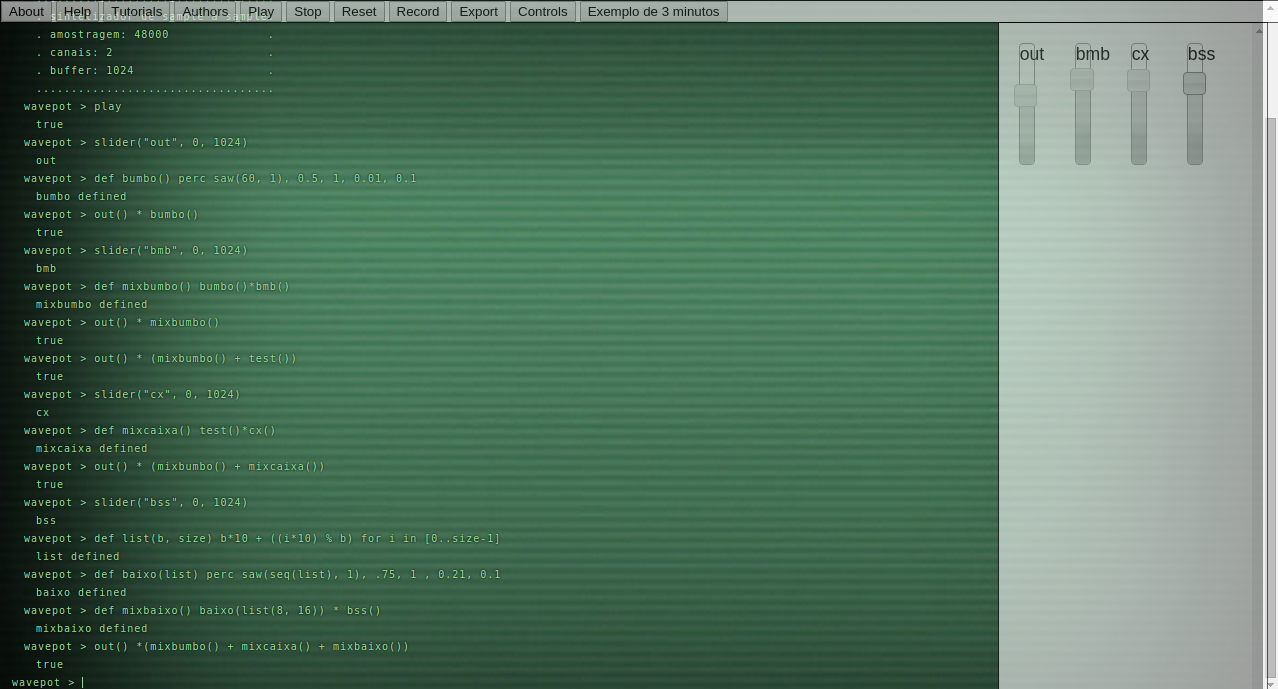
\includegraphics[scale=0.35]{termpot.png}
\caption{Aplicativo \emph{Termpot}. \textbf{Fonte}: autores.}
\label{fig:termpot}
\end{figure}

\begin{listing}
\begin{minted}[linenos,frame=lines,framesep=2mm,fontsize=\scriptsize]{javascript}
wavepot > slider("left", 0, 1024)
true
wavepot > slider("right", 0, 1024)
true
wavepot > stereo sin(440,0.5)*left(), sin(330, 0.5)*right()
true
\end{minted}
\caption{Exemplo de código do Wavepot}
\label{code:resultado15}
\end{listing}



% ---------------------------------------------------------------------------
\section{Conclusão}\label{sec:conclusao}

Este trabalho tratou de investigar a \emph{Web Audio API} e alguns trabalhos derivados desta API partindo de uma abordagem técnica.
A investigação desta API e suas possibilidades musicais e artísticas levaram ao desenvolvimento de uma ferramenta chamada Termpot.

No processo de desenvolvimento do Termpot levamos em conta um processo de síntese semelhante ao \emph{Wavepot} e realizamos algumas customizações.
Características presentes nos ambientes Gibber e Wavepot que julgamos importantes foram adicionadas a nova ferramenta.
Mesmo rudimentar se comparada a estas ferramentas, a ferramenta desenvolvida apresentou-se bastante versátil.

Entretanto, apontamos os seguintes problemas técnico : a biblioteca jQuery apontada como uma provável fonte de \emph{xruns}\footnote{\emph{Google Chrome} 44.0.2403.89 Ubuntu 14.04. Embora o conceito seja original do ALSA (Linux), o fenômeno é semelhante do ponto de vista perceptivo. Sua definição técnica é: "Um 'xrun' pode ser um estouro de buffer ou de uma saturação de um buffer. Um aplicativo de áudio ou não foi rápido o suficiente para transmitir dados (\ldots) ou não rápido o suficiente para processar os dados" \cite{markc_xruns_2013}. Tradução nossa de \emph{An "xrun" can be either a buffer underrun or a buffer overrun. In both cases an audio app was either not fast enough to deliver data (\ldots)  or not fast enough to process data (\ldots)}.}.

Além disso é discutido na comunidade \emph{WebAudio API} a substituição do 


A criação musical baseada em funções matemáticas, como é proposto na abordagem do Termpot, permite ao músico explorar as técnicas tradicionais de síntese como síntese aditiva, subtrativa, FM, AM mas permite também explorar outras construções musicais que diferem destas técnicas.
Neste sentido, a ferramenta desenvolvida apresenta uma abordagem técnico-composicional diferenciada de alguns métodos e ferramentas existentes por poder estabelecer-se no limiar entre a matemática e a música.



\subsection{Trabalhos Futuros}

\begin{inparaenum}[\itshape i)\upshape]
\item criar um servidor;
\item otimizar o emulador, talvez substituindo o Ptty ou propondo melhorias;
\item suporte para amostras pré-gravadas.
\end{inparaenum}

\footnote{Disponível em  \url{https://jahpd.github.io/termpot}.}. 

\subsection{Agradecimentos}

Os autores agradecem ao Guilherme Rafael Soares por ter apresentado as biblioteca Ptty.js, aos desenvolvedores dos projetos investigados por disponibilizarem seus códigos e a FAPEMIG por subsidiar a pesquisa.

 
\bibliographystyle{sbc}
\bibliography{main}

\end{document}